\documentclass{beamer}

\usetheme{Darmstadt}
%\usetheme{Madrid}
%\usecolortheme[named=Maroon]{structure}
%\usecolortheme{dolphin}
%\usefonttheme{professionalfonts}
\useoutertheme{infolines}
\useinnertheme{circles}

\usepackage{pgfpages}
%\setbeameroption{hide notes} % Only slides
%\setbeameroption{show only notes} % Only notes
\setbeameroption{show notes on second screen=right} % Both
\setbeamertemplate{note page}{\pagecolor{yellow!5}\vfill\insertnote\vfill}

\raggedright


\title{Makerspace Badging Project}
\subtitle{}
\author{Thaddeus Bird Murphy}
%\institute{U New Haven}
\date{\today}

% You should be prepared to discuss a project you've worked on that highlights your qualifications for this position. A brief (10-15 minute) overview will do fine that will lead into questions and discussion. Screen projection and wifi access will be available if desired. Your audience will be primarily technical.
	
\begin{document}
%\beamertemplatenavigationsymbolsempty


\section{Intro}
\begin{frame}
	\titlepage%
\end{frame}

\begin{frame}{Introduction}
	\note{While at University I worked at our Makerspace, a place to create, build, make,. I was a student worker, so I was doing this in addition to other acedemics. We have a lot of different machines and tools for individuals and classes to use for both academic and personal projects. In one day we could get over a hundred different students coming in. My job had a few different tasks, some being communication with professors, but the bulk of it was technological integration with the space. A previous project I had worked on was moving our 3D printing system to the cloud and making sure we could understand the data it gave us.}
	\begin{itemize}
		\item The makerspace is a place to create, build, and make
		\item Many students use the space
		\item The space has a lot of different machines that can be used
		\item The machines require different training to use them safely
	\end{itemize}
\end{frame}

\begin{frame}{Problem Statement}
	\note{Before the implementation of the makerspace badging system, our organization lacked a streamlined method for tracking and monitoring individual training levels on various machinery within the makerspace. This absence of structured oversight posed significant safety concerns and operational inefficiencies, as staff were unable to accurately assess the skill levels of users accessing different equipment. Consequently, there was a heightened risk of accidents and misuse of machinery, potentially resulting in injury or damage to both users and equipment. Additionally, the absence of a centralized system made it challenging to maintain compliance with safety regulations and effectively allocate resources for training initiatives. Thus, there was a critical need for an automated system to effectively manage and monitor training levels, ensuring a safer and more efficient makerspace environment for all users.}
	\begin{itemize}
		\item Tracking user training on machinery was manual and decentralized
		\item This led to safety risks, operational inefficiencies, and regulatory compliance challenges
		\item A centralized system is needed to ensure safety, streamline operations, and improve compliance with University safety guidelines
	\end{itemize}
\end{frame}

\section{The Solution}
\begin{frame}{Solution Overview}
	\note{My solution needed to do a few things. Firstly everything needed to be in one place. We couldn't have random spreadsheets with some info and google forms output with other info. Secondly, there shouldn't be any searching required, rather than looking through a list of names for a specific one, you should be able to give the sytsem a name and it has everything right there. And finally staff should not need extensive training to learn to use the system. Someone should be able to learn to use it in a few minutes.}
	\begin{itemize}
		\item Have a central repository of student training levels
		\item Make the information easily and quickly accessable
		\item Low barrier to entry to use
	\end{itemize}
\end{frame}

\begin{frame}{Scope}
	\note{I had a fairly limited time to work on this project with other university work and other makerspace duties, so I had to plan around that. This was all done in my final semester as a senior with my academics taking priority. The secondary goal of this project was for me to learn so I was not going to just go out and find some Software as a Service solution. And while we do have a lot of students using the makerspace, even over a multiyear period that will not exceed thousands.}
	\begin{itemize}
		\item Fairly small scope due to time constrains
		\item To facilitate learning on my part, project should be built from the ground up
		\item Does not need to scale to more than thousands of students tracked
	\end{itemize}
\end{frame}

\begin{frame}{Technical Details}
	\note{My solution is based upon the fact that all students have a student ID, which all have a barcode, magstrip, and NFC all storing a unique to that student string. This basis will make the system very easy to use as everyone already knows how to use their student ID for scanning in to buildings, and there is no issue with two people having the same name.
	My choice for language was mainly off of what I already knew and it is the same with my choice of database. Most of my classes had mainly utilized C++ and the databases class I took was based off of MySQL, which MariaDB is based on
	Finally, if I have the time at the end, I planned on learning how to use Qt to build a GUI front end, rather than a command line interface
	The design itself was fairly straight forward, have an application that queried a database for data on a student, and that could add or modify any of the data.
	}
	\begin{itemize}
		\item Barcode scanner, magstrip reader, and/or NFC reader
		\item C++
		\item MariaDB with MariaDB C++ Connector
		\item If time allowed, Qt frontend
	\end{itemize}
\end{frame}

\section{Outcomes}
\begin{frame}{Process}
	\note{Sadly, those time constrains were more constraining than I expected. I spent a lot of time just whiteboarding ideas and different ways and layouts for how I wanted things to work. If you want to look closely at these pictures there will be a QR code at the end with this entire presentation. Designing the database layout took the most time and I redid it at least twice.}
	\begin{figure}
		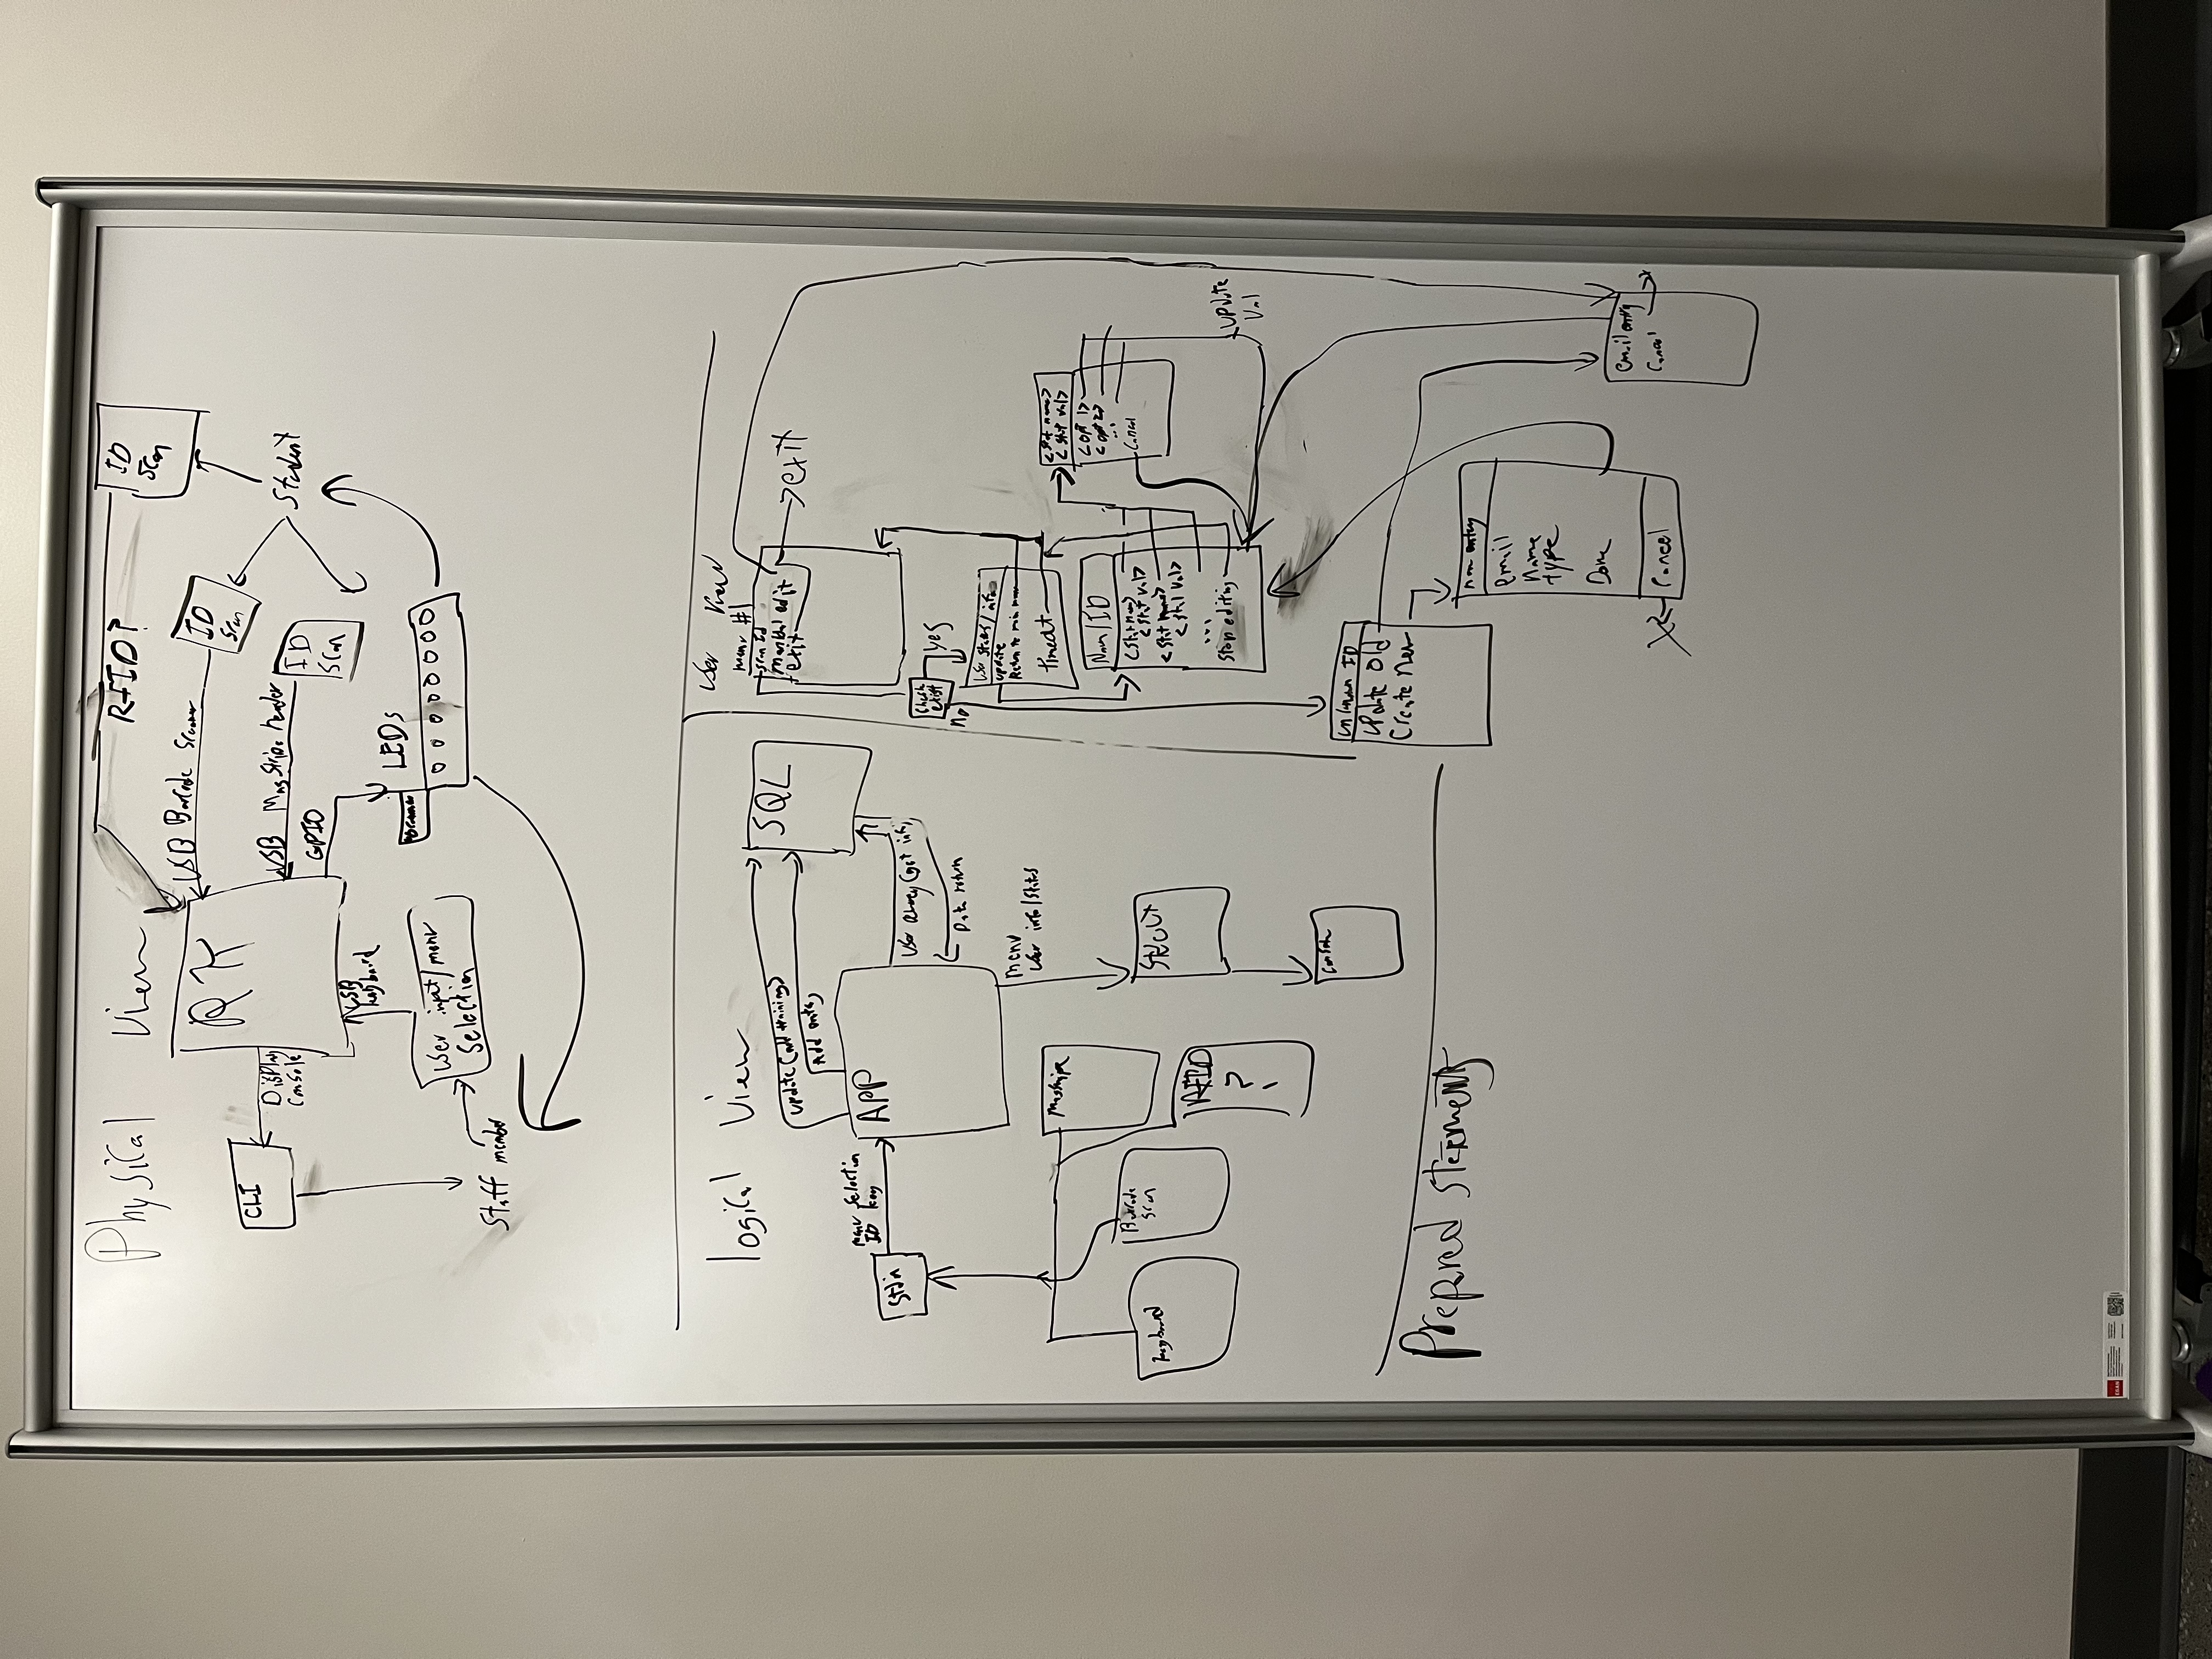
\includegraphics[angle=270,width=0.25\textwidth]{./img/IMG_0143.jpg}
		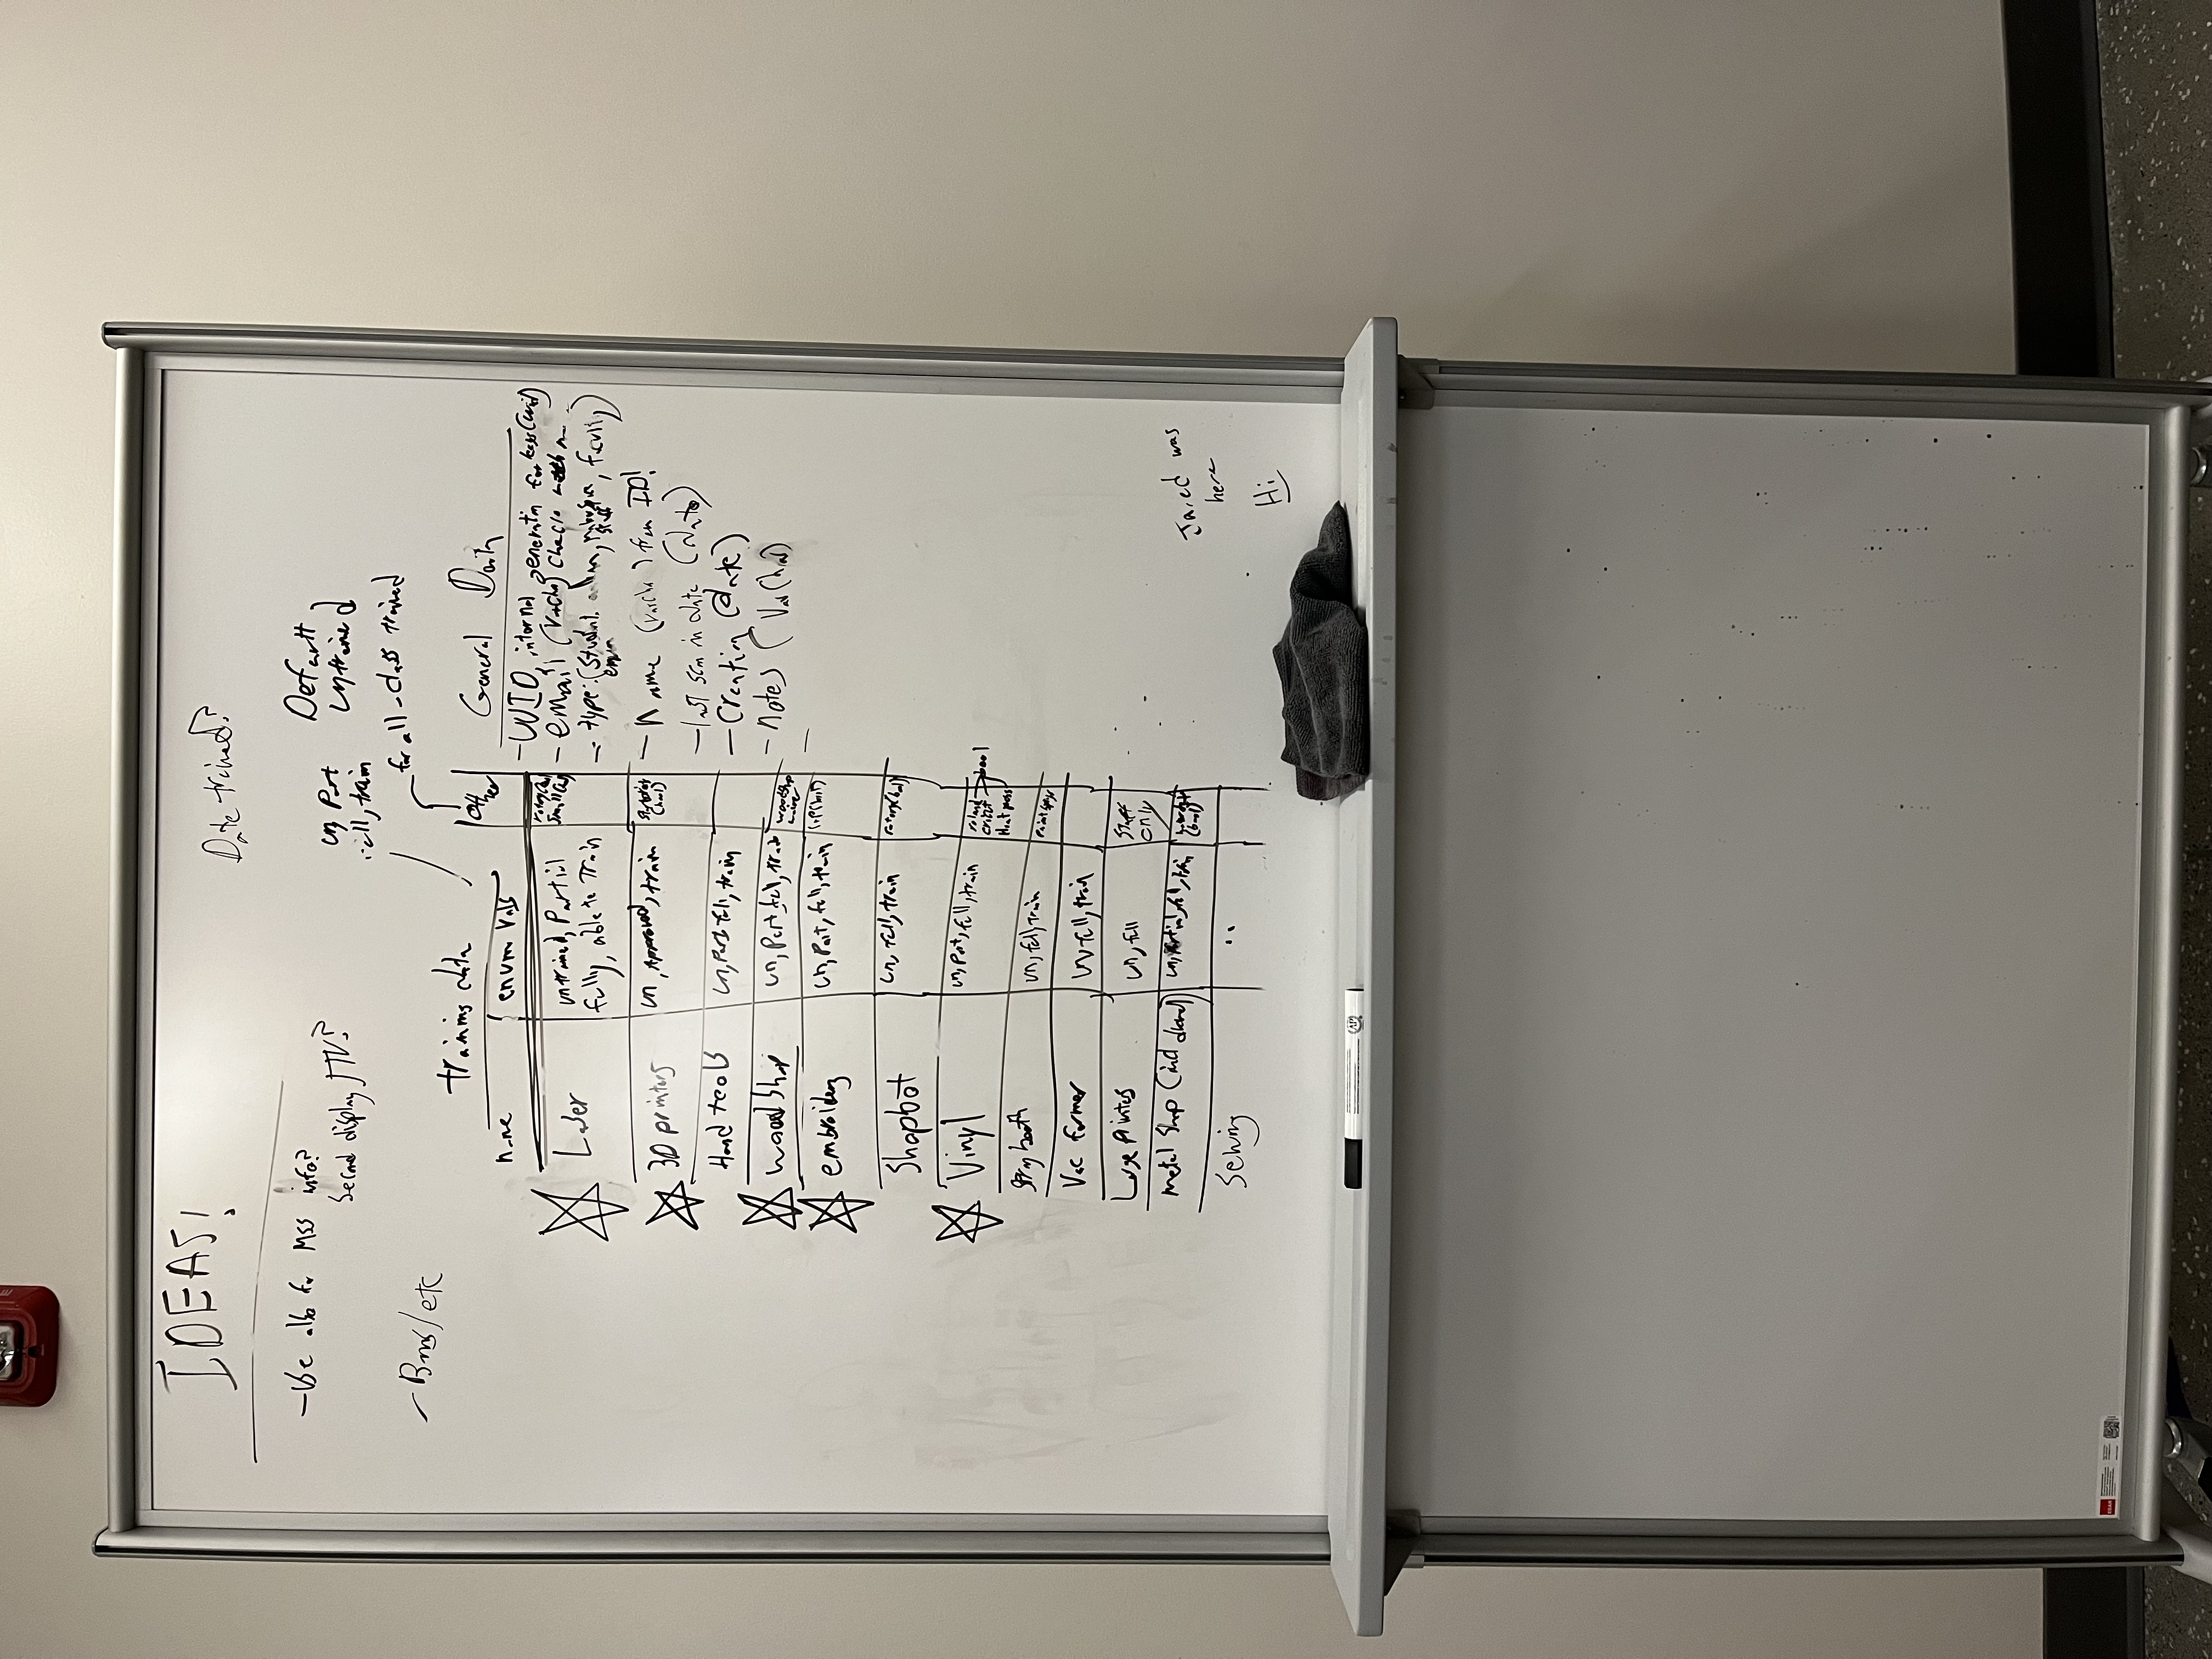
\includegraphics[angle=270,width=0.25\textwidth]{./img/IMG_0144.jpg}
		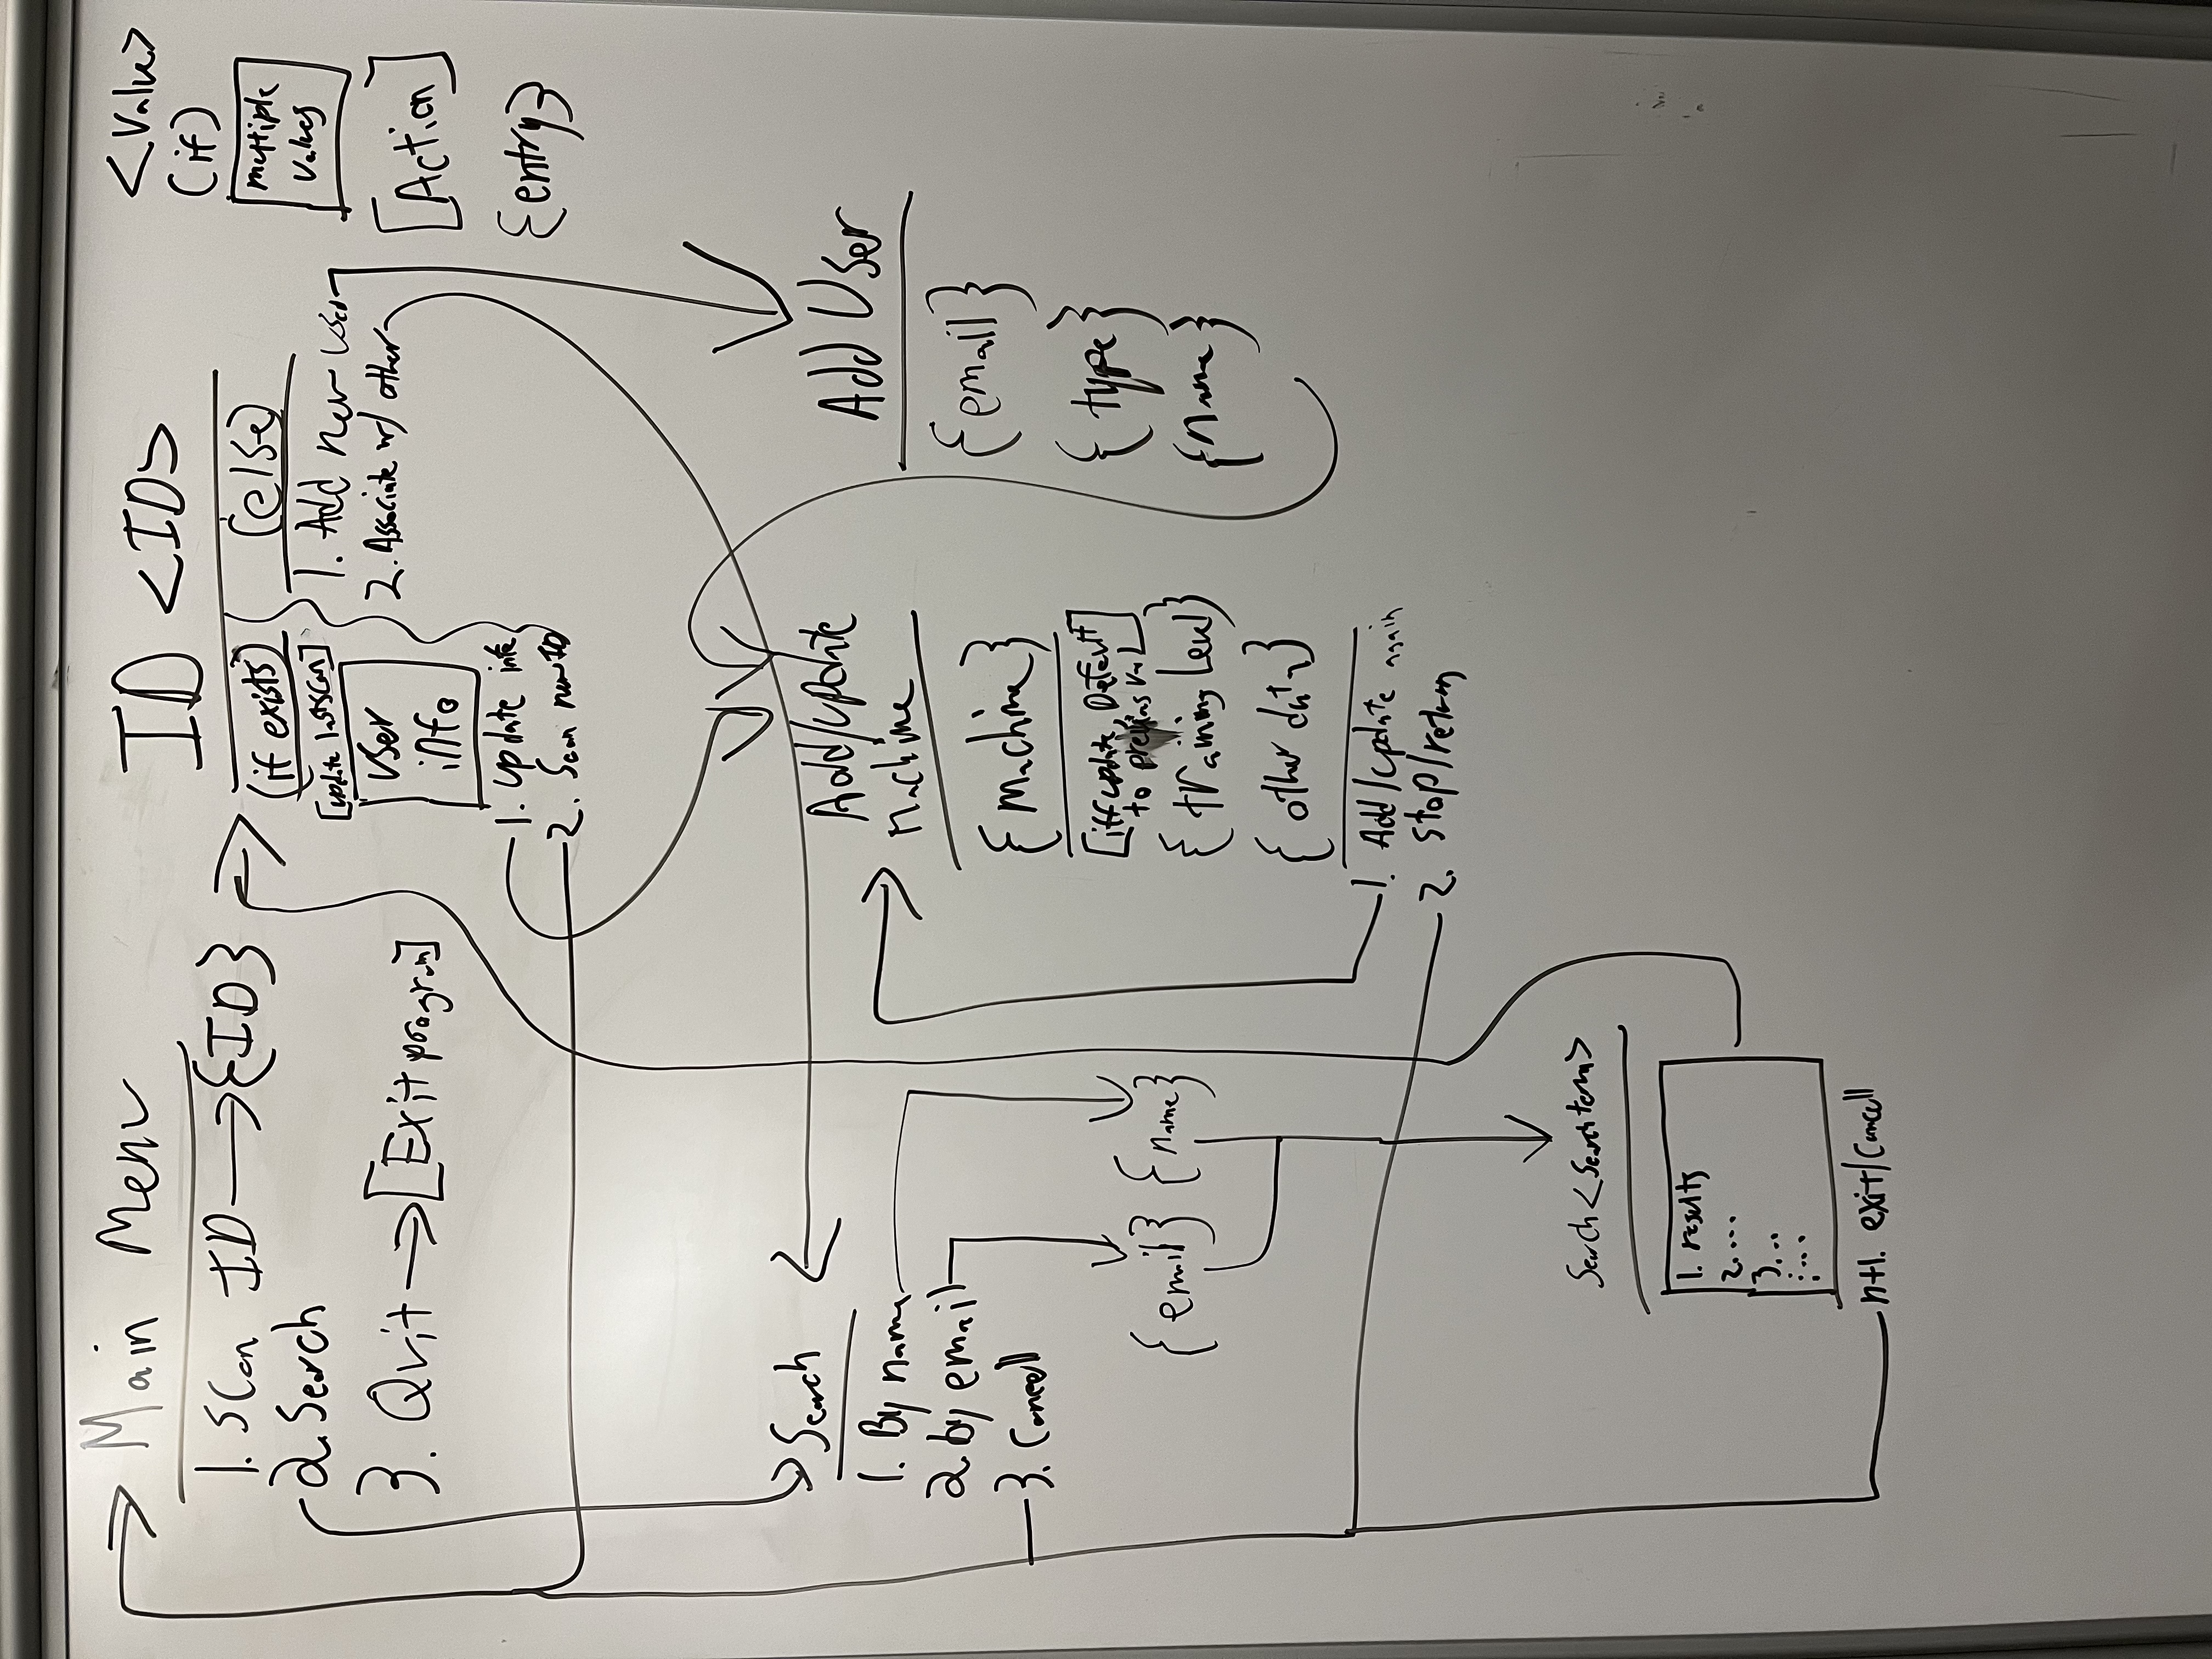
\includegraphics[angle=270,width=0.25\textwidth]{./img/IMG_0216.jpg}
	\end{figure}
\end{frame}
\begin{frame}{Product output/TODO}
	\note{In all I finished the entire database design and how the application would connect to it; I created the CLI menu system and was in the process of implementing the entirety of the CLI user interface when I ran out of time and graduated.}
	\begin{centering}
		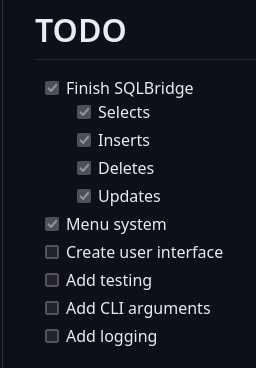
\includegraphics[width=0.33\textwidth]{./img/TODO.png}
	\end{centering}
\end{frame}

\begin{frame}{Reflection/What I would do differently}
	\note{I learned a lot doing this project. The main thing I would change would be how I designed the database. I made this application extremely dependent on how the database worked internally, and I would change this to instead have the application just access an API that would then deal with the data handling and storage itself, abstracting everything out of this one application. Next would be to entirely ditch the CLI idea and just go with Qt or any other graphical library. Trying to do multiphased development where I switch the frontend lead to wasted time on things that were planned to be replaced. Next, a lot of time was lost with a lot of manual testing of components, but no central verification that everything works as expected. }
	\begin{centering}
		\begin{itemize}
			\item Create an API for data retrival
			\item Create a GUI at the start 
			\item Be more test driven
		\end{itemize}
	\end{centering}
\end{frame}

\section{Questions}
\begin{frame}{Questions, comments, etc}
	\begin{figure}
		\centering
		\caption{GitHub Repository (including this presentation)}
			
\includegraphics[width=0.6\textwidth]{./QRCode.eps}
	\end{figure}
\end{frame}
\end{document}
